\documentclass{article}
\usepackage{geometry} %调整页面边距
\usepackage{amsmath}
\usepackage{times}
\usepackage{float}
\usepackage{makecell}
\usepackage{array} % 表格线
\usepackage{booktabs} %调整表格线间隔
\usepackage{enumerate}
\usepackage{graphicx}
\usepackage{caption}
\usepackage{subcaption}
\geometry{left=3.18cm, right=3.18cm, top=2.54cm, bottom=2.54cm}
\begin{document}
\section*{Experiments Outline}

\begin{table}[H]
    \renewcommand{\arraystretch}{1} % default is 1.0
    \centering
    \begin{tabular}{p{3.4cm}p{6.5cm}p{1.1cm}}
        \specialrule{0.05em}{0.5pt}{0.5pt} % 通过插入表格线来控制行高
        \multicolumn{2}{l}{\textbf{Basic parameter settings}} & \textbf{Unit}\\ \hline
        Boarding rate & $\beta=30$                            & pas/min      \\ \hline
        Alighting rate & $\alpha=40$                          & pas/min      \\  \hline
        The minimum headway & $\varepsilon=0.1$               & pas/min      \\ \hline
        Disturbance & \makecell[l]{$delay=2$  occurs in the $51^{st}$ bus of line 1\\ 
                    in the travel link from stop 1 to stop 2} &min           \\ \hline
    \end{tabular}
\end{table}

\newpage

\section{Effect of transfer behavior}

\begin{table}[H]
    \caption*{Experiment 1}
    \label{exp:1}
    \renewcommand{\arraystretch}{1.1} % default is 1.0
    \centering
    \begin{tabular}{p{3.4cm}p{6.5cm}p{1.1cm}}
        \specialrule{0.05em}{0.5pt}{0.5pt} % 通过插入表格线来控制行高
        \textbf{Parameter settings} & \makecell[l]{~}&\textbf{Unit}\\ \hline
        Network & \makecell[l]{$\mathcal{N}_{up}^{1}=\left\{1,2\right\}$, $\mathcal{N}_{up}^{2}=\left\{3,4\right\}$, $\mathcal{N}_{com}^{1,2}=\left\{5,6\right\}$,\\
        $\mathcal{N}_{down}^{1}=\left\{7,8\right\}$, $\mathcal{N}_{down}^{2}=\left\{9,10\right\}$}& 
        \\ \hline
        Bus departure timetable & $H^{1}=H^{2}=6$, $t^{1}=0,t^{2}=3$ & min  
        \\  \hline
        Passenger demand &$\Lambda_{n}=5$, $\forall n\in \mathcal{S}^{1}\cup\mathcal{S}^{2}\backslash\left\{8,10\right\}$&pas/min
        \\ \hline
        Transfer parameter & $\mu=1$&  
        \\ \hline
        Travel times & \makecell[l]{$T_{m,n}=3$,\\  $\forall m\in\mathcal{M}^{1}\cup \mathcal{M}^{2},n\in \mathcal{S}^{1}\cup\mathcal{S}^{2}\backslash \left\{8,10\right\}$}& min\\ \hline
        Capacity & $cap_m=100$, $\forall m\in\mathcal{M}^{1}\cup \mathcal{M}^{2}$&pas 
        \\ \hline
        \makecell[l]{Assignment of transfer\\passengers} & MSA ($k=1$)&
        % \multicolumn{1}{@{}c@{}|}
        % {\begin{tabular}{c|c}
        % MSA & f 
        % \end{tabular}}
        \\ \hline
    \end{tabular}
\end{table}

\begin{figure}[H]
    \centering
    \begin{tabular}{cc}
        \subfloat[Undisturbed bus trajectories]{\includegraphics[width=0.4\textwidth]{experiments/experiment 1:undisturbed trajectories.png}}
        &\subfloat[Disturbed bus trajectories]{\includegraphics[width=0.4\textwidth]{experiments/experiment 1:disturbed trajectories.png}}\\
        \subfloat[MSA $\alpha$ from line 1 to line 2]{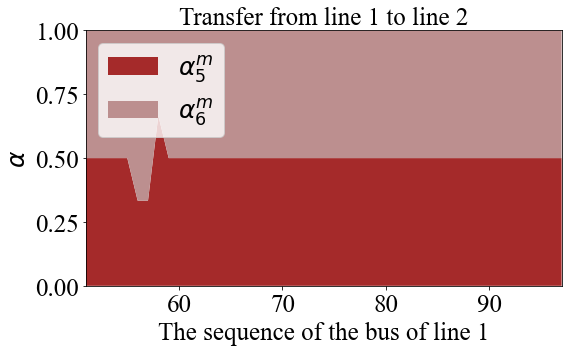
\includegraphics[width=0.4\textwidth]{experiments/experiment 1:MSA alpha 1 to 2.png}}
        &\subfloat[MSA $\alpha$ from line 2 to line 1]{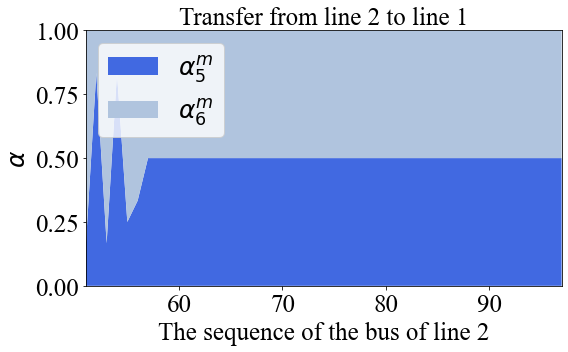
\includegraphics[width=0.4\textwidth]{experiments/experiment 1:MSA alpha 2 to 1.png}}\\
        \subfloat[Heatmap of deviation times of bus dwell events of line 1]{\includegraphics[width=0.3\textwidth]{experiments/experiment 1:affected bus dwell events of line 1.png}}
        &\subfloat[Heatmap of deviation times of bus dwell events of line 2]{\includegraphics[width=0.3\textwidth]{experiments/experiment 1:affected bus dwell events of line 2.png}}                 
        \end{tabular}
        \caption{Experiment 1}
        \label{fig:experiment 1}
    \end{figure}

\begin{table}[H]
    \caption*{Experiment 2}
    \renewcommand{\arraystretch}{1.1} % default is 1.0
    \centering
    \begin{tabular}{p{3.4cm}p{6.5cm}p{1.1cm}}
        \specialrule{0.05em}{0.5pt}{0.5pt} % 通过插入表格线来控制行高
        \textbf{Parameter settings} & \makecell[l]{~}&\textbf{Unit}
        \\ \hline
        Network & \makecell[l]{$\mathcal{N}_{up}^{1}=\left\{1,2\right\}$, $\mathcal{N}_{up}^{2}=\left\{3,4\right\}$, $\mathcal{N}_{com}^{1,2}=\left\{5,6\right\}$,\\
        $\mathcal{N}_{down}^{1}=\left\{7,8\right\}$, $\mathcal{N}_{down}^{2}=\left\{9,10\right\}$}& 
        \\ \hline
        Bus departure timetable & $H^{1}=H^{2}=6$, $t^{1}=0,t^{2}=3$ & min  
        \\  \hline
        Passenger demand &$\Lambda_{n}=5$, $\forall n\in \mathcal{S}^{1}\cup\mathcal{S}^{2}\backslash\left\{8,10\right\}$&pas/min
        \\ \hline
        Transfer parameter & $\mu=1$&  
        \\ \hline
        Travel times & \makecell[l]{$T_{m,n}=3$,\\  $\forall m\in\mathcal{M}^{1}\cup \mathcal{M}^{2},n\in \mathcal{S}^{1}\cup\mathcal{S}^{2}\backslash \left\{8,10\right\}$}& min
        \\ \hline
        Capacity & $cap_m=100$, $\forall m\in\mathcal{M}^{1}\cup \mathcal{M}^{2}$&pas 
        \\ \hline
        \makecell[l]{Assignment of transfer\\passengers} & Equal assignment
        % \makecell[l]{$\alpha_{n_i}^{m} = \frac{1}{\left|\mathcal{N}_{com}^{1,2}\right|}, \forall i=1,...,\left|\mathcal{N}_{com}^{1,2}\right|$;\\
        % $m\in \mathcal{M}^{1}\cup\mathcal{M}^{2}$} 
        &\\ \hline
    \end{tabular}
\end{table}

\begin{figure}[H]
    \centering
    \begin{tabular}{cc}
        \subfloat[Undisturbed bus trajectories]{\includegraphics[width=0.4\textwidth]{experiments/experiment 2:undisturbed trajectories.png}}
        &\subfloat[Disturbed bus trajectories]{\includegraphics[width=0.4\textwidth]{experiments/experiment 2:disturbed trajectories.png}}\\
        \subfloat[Equal $\alpha$ from line 1 to line 2]{\includegraphics[width=0.4\textwidth]{experiments/experiment 2:equal alpha 1 to 2.png}}
        &\subfloat[Equal $\alpha$ from line 2 to line 1]{\includegraphics[width=0.4\textwidth]{experiments/experiment 2:equal alpha 2 to 1.png}}\\
        \subfloat[Heatmap of deviation times of bus dwell events of line 1]{\includegraphics[width=0.3\textwidth]{experiments/experiment 2:affected bus dwell events of line 1.png}}
        &\subfloat[Heatmap of deviation times of bus dwell events of line 2]{\includegraphics[width=0.3\textwidth]{experiments/experiment 2:affected bus dwell events of line 2.png}}                 
        \end{tabular}
        \caption{Experiment 2}
        \label{fig:experiment 2}
    \end{figure}

\begin{table}[H]
    \caption*{Experiment 3}
    \renewcommand{\arraystretch}{1.1} % default is 1.0
    \centering
    \begin{tabular}{p{3.4cm}p{6.5cm}p{1.1cm}}
        \specialrule{0.05em}{0.5pt}{0.5pt} % 通过插入表格线来控制行高
        \textbf{Parameter settings} & \makecell[l]{~}&\textbf{Unit}
        \\ \hline
        Network & \makecell[l]{$\mathcal{N}_{up}^{1}=\left\{1,2\right\}$, $\mathcal{N}_{up}^{2}=\left\{3,4\right\}$, $\mathcal{N}_{com}^{1,2}=\left\{5,6\right\}$,\\
        $\mathcal{N}_{down}^{1}=\left\{7,8\right\}$, $\mathcal{N}_{down}^{2}=\left\{9,10\right\}$}& 
        \\ \hline
        Bus departure timetable & $H^{1}=H^{2}=6$, $t^{1}=0,t^{2}=3$ & min  
        \\  \hline
        Passenger demand &$\Lambda_{n}=5$, $\forall n\in \mathcal{S}^{1}\cup\mathcal{S}^{2}\backslash\left\{8,10\right\}$&pas/min
        \\ \hline
        Transfer parameter & $\mu=0$&  
        \\ \hline
        Travel times & \makecell[l]{$T_{m,n}=3$,\\  $\forall m\in\mathcal{M}^{1}\cup \mathcal{M}^{2},n\in \mathcal{S}^{1}\cup\mathcal{S}^{2}\backslash \left\{8,10\right\}$}& min
        \\ \hline
        Capacity & $cap_m=100$, $\forall m\in\mathcal{M}^{1}\cup \mathcal{M}^{2}$&pas 
        \\ \hline
        \makecell[l]{Assignment of transfer\\passengers} & Equal assignment
        &\\ \hline
    \end{tabular}
\end{table}

\begin{figure}[H]
    \centering
    \begin{tabular}{cc}
        \subfloat[Undisturbed bus trajectories]{\includegraphics[width=0.4\textwidth]{experiments/experiment 3:undisturbed trajectories.png}}
        &\subfloat[Disturbed bus trajectories]{\includegraphics[width=0.4\textwidth]{experiments/experiment 3:disturbed trajectories.png}}\\
        \subfloat[Heatmap of deviation times of bus dwell events of line 1]{\includegraphics[width=0.3\textwidth]{experiments/experiment 3:affected bus dwell events of line 1.png}}
        &\subfloat[Heatmap of deviation times of bus dwell events of line 2]{\includegraphics[width=0.3\textwidth]{experiments/experiment 3:affected bus dwell events of line 2.png}}                 
        \end{tabular}
        \caption{Experiment 3}
        \label{fig:experiment 3}
    \end{figure}

\begin{table}[H]
    \caption*{Experiment 4}
    \renewcommand{\arraystretch}{1.1} % default is 1.0
    \centering
    \begin{tabular}{p{3.4cm}p{6.5cm}p{1.1cm}}
        \specialrule{0.05em}{0.5pt}{0.5pt} % 通过插入表格线来控制行高
        \textbf{Parameter settings} & \makecell[l]{~}&\textbf{Unit}
        \\ \hline
        Network & \makecell[l]{$\mathcal{N}_{up}^{1}=\left\{1,2\right\}$, $\mathcal{N}_{up}^{2}=\left\{3,4\right\}$, $\mathcal{N}_{com}^{1,2}=\left\{5,6\right\}$,\\
        $\mathcal{N}_{down}^{1}=\left\{7,8\right\}$, $\mathcal{N}_{down}^{2}=\left\{9,10\right\}$}& 
        \\ \hline
        Bus departure timetable & $H^{1}=H^{2}=6$, $t^{1}=0,t^{2}=3$ & min  
        \\  \hline
        Passenger demand &$\Lambda_{n}=5$, $\forall n\in \mathcal{S}^{1}\cup\mathcal{S}^{2}\backslash\left\{8,10\right\}$&pas/min
        \\ \hline
        Transfer parameter & $\mu=5$&  
        \\ \hline
        Travel times & \makecell[l]{$T_{m,n}=3$,\\  $\forall m\in\mathcal{M}^{1}\cup \mathcal{M}^{2},n\in \mathcal{S}^{1}\cup\mathcal{S}^{2}\backslash \left\{8,10\right\}$}& min
        \\ \hline
        Capacity & $cap_m=100$, $\forall m\in\mathcal{M}^{1}\cup \mathcal{M}^{2}$&pas 
        \\ \hline
        \makecell[l]{Assignment of transfer\\passengers} & Equal assignment
        &\\ \hline
    \end{tabular}
\end{table}

\begin{figure}[H]
    \centering
    \begin{tabular}{cc}
        \subfloat[Undisturbed bus trajectories]{\includegraphics[width=0.4\textwidth]{experiments/experiment 4:undisturbed trajectories.png}}
        &\subfloat[Disturbed bus trajectories]{\includegraphics[width=0.4\textwidth]{experiments/experiment 4:disturbed trajectories.png}}\\
        \subfloat[Heatmap of deviation times of bus dwell events of line 1]{\includegraphics[width=0.3\textwidth]{experiments/experiment 4:affected bus dwell events of line 1.png}}
        &\subfloat[Heatmap of deviation times of bus dwell events of line 2]{\includegraphics[width=0.3\textwidth]{experiments/experiment 4:affected bus dwell events of line 2.png}}                 
        \end{tabular}
        \caption{Experiment 4}
        \label{fig:experiment 4}
    \end{figure}

\section{Effect of capacity constraint}
\begin{table}[H]
    \caption*{Experiment 5}
    \renewcommand{\arraystretch}{1.1} % default is 1.0
    \centering
    \begin{tabular}{p{3.4cm}p{6.5cm}p{1.1cm}}
        \specialrule{0.05em}{0.5pt}{0.5pt} % 通过插入表格线来控制行高
        \textbf{Parameter settings} & \makecell[l]{~}&\textbf{Unit}
        \\ \hline
        Network & \makecell[l]{$\mathcal{N}_{up}^{1}=\left\{1,2\right\}$, $\mathcal{N}_{up}^{2}=\left\{3,4\right\}$, $\mathcal{N}_{com}^{1,2}=\left\{5,6\right\}$,\\
        $\mathcal{N}_{down}^{1}=\left\{7,8\right\}$, $\mathcal{N}_{down}^{2}=\left\{9,10\right\}$}& 
        \\ \hline
        Bus departure timetable & $H^{1}=H^{2}=6$, $t^{1}=0,t^{2}=3$ & min  
        \\  \hline
        Passenger demand &$\Lambda_{n}=6$, $\forall n\in \mathcal{S}^{1}\cup\mathcal{S}^{2}\backslash\left\{8,10\right\}$&pas/min
        \\ \hline
        Transfer parameter & $\mu=1$&  
        \\ \hline
        Travel times & \makecell[l]{$T_{m,n}=3$,\\  $\forall m\in\mathcal{M}^{1}\cup \mathcal{M}^{2},n\in \mathcal{S}^{1}\cup\mathcal{S}^{2}\backslash \left\{8,10\right\}$}& min
        \\ \hline
        Capacity & $cap_m=150$, $\forall m\in\mathcal{M}^{1}\cup \mathcal{M}^{2}$&pas 
        \\ \hline
        \makecell[l]{Assignment of transfer\\passengers} & Equal assignment
        &\\ \hline
    \end{tabular}
\end{table}

\begin{figure}[H]
    \centering
    \begin{tabular}{cc}
        \subfloat[Undisturbed bus trajectories]{\includegraphics[width=0.4\textwidth]{experiments/experiment 5:undisturbed trajectories.png}}
        &\subfloat[Disturbed bus trajectories]{\includegraphics[width=0.4\textwidth]{experiments/experiment 5:disturbed trajectories.png}}\\
        \subfloat[Heatmap of deviation times of bus dwell events of line 1]{\includegraphics[width=0.3\textwidth]{experiments/experiment 5:affected bus dwell events of line 1.png}}
        &\subfloat[Heatmap of deviation times of bus dwell events of line 2]{\includegraphics[width=0.3\textwidth]{experiments/experiment 5:affected bus dwell events of line 2.png}}                 
        \end{tabular}
        \caption{Experiment 5}
        \label{fig:experiment 5}
    \end{figure}

    \begin{table}[H]
        \caption*{Experiment 6}
        \renewcommand{\arraystretch}{1.1} % default is 1.0
        \centering
        \begin{tabular}{p{3.4cm}p{6.5cm}p{1.1cm}}
            \specialrule{0.05em}{0.5pt}{0.5pt} % 通过插入表格线来控制行高
            \textbf{Parameter settings} & \makecell[l]{~}&\textbf{Unit}
            \\ \hline
            Network & \makecell[l]{$\mathcal{N}_{up}^{1}=\left\{1,2\right\}$, $\mathcal{N}_{up}^{2}=\left\{3,4\right\}$, $\mathcal{N}_{com}^{1,2}=\left\{5,6\right\}$,\\
            $\mathcal{N}_{down}^{1}=\left\{7,8\right\}$, $\mathcal{N}_{down}^{2}=\left\{9,10\right\}$}& 
            \\ \hline
            Bus departure timetable & $H^{1}=H^{2}=6$, $t^{1}=0,t^{2}=3$ & min  
            \\  \hline
            Passenger demand &$\Lambda_{n}=6$, $\forall n\in \mathcal{S}^{1}\cup\mathcal{S}^{2}\backslash\left\{8,10\right\}$&pas/min
            \\ \hline
            Transfer parameter & $\mu=1$&  
            \\ \hline
            Travel times & \makecell[l]{$T_{m,n}=3$,\\  $\forall m\in\mathcal{M}^{1}\cup \mathcal{M}^{2},n\in \mathcal{S}^{1}\cup\mathcal{S}^{2}\backslash \left\{8,10\right\}$}& min
            \\ \hline
            Capacity & $cap_m=80$, $\forall m\in\mathcal{M}^{1}\cup \mathcal{M}^{2}$&pas 
            \\ \hline
            \makecell[l]{Assignment of transfer\\passengers} & Equal assignment
            &\\ \hline
        \end{tabular}
    \end{table}
    
    \begin{figure}[H]
        \centering
        \begin{tabular}{cc}
            \subfloat[Undisturbed bus trajectories]{\includegraphics[width=0.4\textwidth]{experiments/experiment 6:undisturbed trajectories.png}}
            &\subfloat[Disturbed bus trajectories]{\includegraphics[width=0.4\textwidth]{experiments/experiment 6:disturbed trajectories.png}}\\
            \subfloat[Heatmap of deviation times of bus dwell events of line 1]{\includegraphics[width=0.3\textwidth]{experiments/experiment 6:affected bus dwell events of line 1.png}}
            &\subfloat[Heatmap of deviation times of bus dwell events of line 2]{\includegraphics[width=0.3\textwidth]{experiments/experiment 6:affected bus dwell events of line 2.png}}                 
            \end{tabular}
            \caption{Experiment 6}
            \label{fig:experiment 6}
        \end{figure}

        \begin{table}[H]
            \caption*{Experiment 7}
            \renewcommand{\arraystretch}{1.1} % default is 1.0
            \centering
            \begin{tabular}{p{3.4cm}p{6.5cm}p{1.1cm}}
                \specialrule{0.05em}{0.5pt}{0.5pt} % 通过插入表格线来控制行高
                \textbf{Parameter settings} & \makecell[l]{~}&\textbf{Unit}
                \\ \hline
                Network & \makecell[l]{$\mathcal{N}_{up}^{1}=\left\{1,2\right\}$, $\mathcal{N}_{up}^{2}=\left\{3,4\right\}$, $\mathcal{N}_{com}^{1,2}=\left\{5,6\right\}$,\\
                $\mathcal{N}_{down}^{1}=\left\{7,8\right\}$, $\mathcal{N}_{down}^{2}=\left\{9,10\right\}$}& 
                \\ \hline
                Bus departure timetable & $H^{1}=6$,$H^{2}=3$, $t^{1}=0,t^{2}=1.5$ & min  
                \\  \hline
                Passenger demand &$\Lambda_{n}=5$, $\forall n\in \mathcal{S}^{1}\cup\mathcal{S}^{2}\backslash\left\{8,10\right\}$&pas/min
                \\ \hline
                Transfer parameter & $\mu=1$&  
                \\ \hline
                Travel times & \makecell[l]{$T_{m,n}=3$,\\  $\forall m\in\mathcal{M}^{1}\cup \mathcal{M}^{2},n\in \mathcal{S}^{1}\cup\mathcal{S}^{2}\backslash \left\{8,10\right\}$}& min
                \\ \hline
                Capacity & $cap_m=150$, $\forall m\in\mathcal{M}^{1}\cup \mathcal{M}^{2}$&pas 
                \\ \hline
                \makecell[l]{Assignment of transfer\\passengers} & MSA assignment
                &\\ \hline
            \end{tabular}
        \end{table}
        
        \begin{figure}[H]
            \centering
            \begin{tabular}{cc}
                \subfloat[Undisturbed bus trajectories]{\includegraphics[width=0.4\textwidth]{experiments/experiment 6:undisturbed trajectories.png}}
                &\subfloat[Disturbed bus trajectories]{\includegraphics[width=0.4\textwidth]{experiments/experiment 6:disturbed trajectories.png}}\\
                \subfloat[Heatmap of deviation times of bus dwell events of line 1]{\includegraphics[width=0.3\textwidth]{experiments/experiment 6:affected bus dwell events of line 1.png}}
                &\subfloat[Heatmap of deviation times of bus dwell events of line 2]{\includegraphics[width=0.3\textwidth]{experiments/experiment 6:affected bus dwell events of line 2.png}}                 
                \end{tabular}
                \caption{Experiment 7}
                \label{fig:experiment 7}
            \end{figure}
\end{document}